\chapter{Specifikacija programske potpore}
		
	\section{Funkcionalni zahtjevi}
			
			\noindent \textbf{Dionici:}
			
			\begin{packed_enum}
				
				\item Natjecatelj
				\item Voditelj
				\item Administrator				
				\item Razvojni tim
				
			\end{packed_enum}
			
			\noindent \textbf{Aktori i njihovi funkcionalni zahtjevi:}
			
			
			\begin{packed_enum}
				\item  \underbar{Neregistrirani/neprijavljeni korisnik (inicijator) može:}
				
				\begin{packed_enum}
					
					\item pretraživati natjecanja i pristupiti popisu zadataka s natjecanja i sudionika natjecanja
					\item pretraživati i čitati zadatke s natjecanja
					\item pristupiti informacijama tuđeg korisničkog profila:
					
					\begin{packed_enum}
						
					\item  korisničko ime, ime i prezime, i osvojene nagrade
					\item  statistike u što se ubraja broj točno riješenih i broj isprobanih zadataka
					\item  popis natjecanja na kojima je korisnik prisustvovao ili natjecanja koja je održavao
					
				
					\end{packed_enum}
					\item se registrirati u sustav, stvoriti novi korisnički račun za koji:
					
					\begin{packed_enum}
						
						\item  su mu potrebni korisničko ime, lozinka, ime i prezime te e-mail adresa
						\item  mora izabrati razinu pristupa "natjecatelj" ili "voditelj"
						
					\end{packed_enum}
				\end{packed_enum}
			
				\item  \underbar{Natjecatelj (inicijator) može:}
				
				\begin{packed_enum}
					
					\item pregledavati i mijenjati osobne podatke
					\item izbrisati svoj korisnički račun
					\item pristupiti zadatcima za vježbu i rješavati ih
					\item prijaviti i odjaviti se na natjecanja i pristupiti natjecanjima
					\item osvojiti nagrade
					\item pokrenuti virtualno natjecanje
					
				\end{packed_enum}
			
				\item  \underbar{Voditelj (inicijator) može:}
				
				\begin{packed_enum}
					
					\item pregledavati i mijenjati osobne podatke
					\item izbrisati svoj korisnički račun
					\item pristupiti zadatcima za vježbu i rješavati ih
					\item prijaviti i odjaviti se na natjecanja i pristupiti natjecanjima
					\item osvojiti nagrade
					\item pokrenuti virtualno natjecanje
					\item pokrenuti i voditi natjecanje 
					\item kreirati  zadatke 
					\item mijenjati i brisati vlastite zadatke
					
				\end{packed_enum}
				
				\item  \underbar{Administrator (inicijator) može:}
				
				\begin{packed_enum}
					
					\item pristupiti zadatcima za vježbu i rješavati ih
					\item prijaviti i odjaviti se na natjecanja i pristupiti natjecanjima
					\item osvojiti nagrade
					\item pokrenuti virtualno natjecanje
					\item pokrenuti i voditi natjecanje 
					\item kreirati  zadatke 
					\item mijenjati vlastite zadatke
					\item vidjeti popis svih registriranih korisnika i njihovih osobnih podataka
					\item korisnike brisati i mijenjati im razinu pristupa aplikaciji (natjecatelj, voditelj, administrator)
					\item pristupiti statistici
					
					
					
				\end{packed_enum}
			
					
			\end{packed_enum}
			
			\eject 
			
			
				
			\subsection{Obrasci uporabe}
				
				\subsubsection{Opis obrazaca uporabe}

				\noindent \underbar{\textbf{UC1 - Registracija}}
					\begin{packed_item}
	
						\item \textbf{Glavni sudionik: } Korisnik
						\item  \textbf{Cilj:} Registracija u sustav
						\item  \textbf{Sudionici:} Baza podataka
						\item  \textbf{Preduvjet:} -
						\item  \textbf{Opis osnovnog tijeka:}
						
						\item[] \begin{packed_enum}
	
							\item Korisnik odabire opciju za registraciju
							\item Korisnik unosi potrebne korisnicke podatke
							\item Korisnik prima obavijest o uspjesnoj registraciji
						\end{packed_enum}
						
						\item  \textbf{Opis mogućih odstupanja:}
						
						\item[] \begin{packed_item}
	
							\item[2.a] Odabir vec zauzetog korisničkog imena i/ili e-maila, unos korisničkog
							podatka u nedozvoljenom formatu ili pruzanje neispravnoga e-maila
							\item[] \begin{packed_enum}
								
								\item Sustav obavještava korisnika o neuspjelom upisu i vraća ga na stra- 
								nicu za registraciju
								\item Korisnik mijenja potrebne podatke te završava unos ili odustaje od 
								registracije
								
							\end{packed_enum}
							
						\end{packed_item}
					\end{packed_item}

					\noindent \underbar{\textbf{UC2 - Prijava}}
					\begin{packed_item}
	
						\item \textbf{Glavni sudionik: } Korisnik
						\item  \textbf{Cilj:} Dobiti pristup korisničkom sučelju
						\item  \textbf{Sudionici:} Baza podataka
						\item  \textbf{Preduvjet:} Registracija
						\item  \textbf{Opis osnovnog tijeka:}
						
						\item[] \begin{packed_enum}
	
							\item Unos korisničkog imena i lozinke
							\item Potvrda o ispravnosti unesenih podataka
							\item Pristup korisničkim funkcijama
						\end{packed_enum}
						
						\item  \textbf{Opis mogućih odstupanja:}
						
						\item[] \begin{packed_item}
	
							\item[2.a] Neispravno korisničko ime/lozinka
							\item[] \begin{packed_enum}
								
								\item Sustav obavještava korisnika o neuspjelom upisu i vraća ga na stra- 
								nicu za registraciju
								
								
							\end{packed_enum}
							
						\end{packed_item}
					\end{packed_item}
					
					\noindent \underbar{\textbf{UC3 - Pregled mojeg profila}}
					\begin{packed_item}
	
						\item \textbf{Glavni sudionik: } Korisnik
						\item  \textbf{Cilj:} Pregledati osobne podatke
						\item  \textbf{Sudionici:} Baza podataka
						\item  \textbf{Preduvjet:} Korisnik je prijavljen
						\item  \textbf{Opis osnovnog tijeka:}
						
						\item[] \begin{packed_enum}
	
							\item Korisnik odabire opciju "Moj Profil"
							\item Aplikacija prikazuje osobne podatke korisnika
						\end{packed_enum}
						
						
					\end{packed_item}

					\noindent \underbar{\textbf{UC4 - Promjena podataka na mojem profilu}}
					\begin{packed_item}
	
						\item \textbf{Glavni sudionik: } Korisnik
						\item  \textbf{Cilj:} Promjeniti osobne podatke
						\item  \textbf{Sudionici:} Baza podataka
						\item  \textbf{Preduvjet:} Korisnik je prijavljen
						\item  \textbf{Opis osnovnog tijeka:}
						
						\item[] \begin{packed_enum}
	
							\item Korisnik odabire opciju "Uredi profil"
							\item Korisnik mijenja svoje osobne podatke
							\item Korisnik sprema promjene
							\item Baza podataka se ažurira
						\end{packed_enum}
						\item  \textbf{Opis mogućih odstupanja:}
						
						\item[] \begin{packed_item}
	
							\item[2.a] Korisnik promjeni svoje osobne podatke, ali ne odabire opciju "Spremi" 
							\item[] \begin{packed_enum}
								
								\item Sustav obavještava korisnika da nije spremio podatke prije izlaza iz prozora.
								
								
							\end{packed_enum}
							
						\end{packed_item}
						
						
					\end{packed_item}

					\noindent \underbar{\textbf{UC5 - Odjava iz sustava}}
					\begin{packed_item}
	
						\item \textbf{Glavni sudionik: } Korisnik
						\item  \textbf{Cilj:} Odjava iz sustava
						\item  \textbf{Sudionici:} Korisnik
						\item  \textbf{Preduvjet:} Korisnik je prijavljen
						\item  \textbf{Opis osnovnog tijeka:}
						
						\item[] \begin{packed_enum}
	
							\item Korisnik odabire opciju "Odjava"
							\item Sustav vraća korisnika na početnu stranicu
						\end{packed_enum}
						
						
					\end{packed_item}

					\noindent \underbar{\textbf{UC6 - Brisanje mojeg profila}}
					\begin{packed_item}
	
						\item \textbf{Glavni sudionik: } Korisnik
						\item  \textbf{Cilj:} Brisanje korisničkog profila
						\item  \textbf{Sudionici:} Baza podataka
						\item  \textbf{Preduvjet:} Korisnik je prijavljen
						\item  \textbf{Opis osnovnog tijeka:}
						
						\item[] \begin{packed_enum}
	
							\item Korisnik odabire opciju "Izbriši Moj Profil"
							\item Sustav odjavljuje korisnika i vraća ga na početnu stranicu
							\item Baza Podataka se ažurira
						\end{packed_enum}
						
						
					\end{packed_item}

					\noindent \underbar{\textbf{UC7 - Pregled zadataka}}
					\begin{packed_item}
	
						\item \textbf{Glavni sudionik: } Korisnik
						\item  \textbf{Cilj:} Pregledati sve dostupne zadatke za vježbu
						\item  \textbf{Sudionici:} Baza podataka
						\item  \textbf{Preduvjet:} -
						\item  \textbf{Opis osnovnog tijeka:}
						
						\item[] \begin{packed_enum}
	
							\item Korisnik odabire opciju "Zadaci"
							\item Korisniku se prikažu svi dostupni zadaci za vježbu
						\end{packed_enum}
						
						
					\end{packed_item}

					\noindent \underbar{\textbf{UC8 - Rješavanje zadataka za vježbu}}
					\begin{packed_item}
	
						\item \textbf{Glavni sudionik: } Korisnik
						\item  \textbf{Cilj:} Pokretanje i rješavanje zadataka za vježbu
						\item  \textbf{Sudionici:} Baza podataka
						\item  \textbf{Preduvjet:} Korisnik je prijavljen
						\item  \textbf{Opis osnovnog tijeka:}
						
						\item[] \begin{packed_enum}
	
							\item Korisnik odabire jedan od zadataka za vježbu
							\item Sustav prebacuje korisnika na stranicu za rješavanje zadataka
						\end{packed_enum}
						
						
					\end{packed_item}

					\noindent \underbar{\textbf{UC9 - Dodavanje zadataka}}
					\begin{packed_item}
	
						\item \textbf{Glavni sudionik: } Voditelj
						\item  \textbf{Cilj:} Dodati novi zadatak u bazu zadataka za vježbu
						\item  \textbf{Sudionici:} Baza podataka
						\item  \textbf{Preduvjet:} Korisnik mora imati ovlasti "Voditelj"
						\item  \textbf{Opis osnovnog tijeka:}
						
						\item[] \begin{packed_enum}
	
							\item Voditelj odabire opciju "Dodaj novi zadatak"
							\item Voditelj upisuje tekst,težinu,rješenje i vremensko ograničenje za zadatak
							\item Voditelj odabire opciju "Završi"
							\item Baza podataka se ažurira
						\end{packed_enum}

						\item  \textbf{Opis mogućih odstupanja:}
						
						\item[] \begin{packed_item}
	
							\item[2.a] Voditelj unosi podatke u nedozvoljenom formatu
							\item[] \begin{packed_enum}
								
								\item Sustav obavještava voditelja o neuspjelom upisu podataka
								\item Voditelj popravlja unose
								
							\end{packed_enum}
						\end{packed_item}
						
						
					\end{packed_item}

					\noindent \underbar{\textbf{UC10 - Pregled sudionika koji su rješavali određeni zadatak}}
					\begin{packed_item}
	
						\item \textbf{Glavni sudionik: } Natjecatelj
						\item  \textbf{Cilj:} Pregledati sudionike koji su rješavali određeni zadatak
						\item  \textbf{Sudionici:} Baza podataka
						\item  \textbf{Preduvjet:} Korisnik je prijavljen
						\item  \textbf{Opis osnovnog tijeka:}
						
						\item[] \begin{packed_enum}
	
							\item Natjecatelj odabire jedan od zadataka
							\item Natjecatelju se otvara lista svih koji su ga rješavali
						\end{packed_enum}
						
						
					\end{packed_item}

					\noindent \underbar{\textbf{UC11 - Brisanje zadataka}}
					\begin{packed_item}
	
						\item \textbf{Glavni sudionik: } Voditelj
						\item  \textbf{Cilj:} Izbrisati zadatak iz baze zadataka za vježbu
						\item  \textbf{Sudionici:} Baza podataka
						\item  \textbf{Preduvjet:} Korisnik mora imati ovlasti "Voditelj"
						\item  \textbf{Opis osnovnog tijeka:}
						
						\item[] \begin{packed_enum}
	
							\item Voditelj odabire jedan od zadataka za vježbu
							\item Voditelj odabire opciju "Izbriši zadatak"
							\item Baza podataka se ažurira
						\end{packed_enum}
						
						
					\end{packed_item}

					\noindent \underbar{\textbf{UC12 - Uređivanje zadataka za vježbu}}
					\begin{packed_item}
	
						\item \textbf{Glavni sudionik: } Voditelj
						\item  \textbf{Cilj:} Urediti zadatak iz baze zadataka za vježbu
						\item  \textbf{Sudionici:} Baza podataka
						\item  \textbf{Preduvjet:} Korisnik mora imati ovlasti "Voditelj"
						\item  \textbf{Opis osnovnog tijeka:}
						
						\item[] \begin{packed_enum}
	
							\item Voditelj odabire jedan od zadataka za vježbu 
							\item Voditelj odabire opciju "Uredi zadatak"
							\item Voditelj upisuje tekst,težinu,rješenje i vremensko ograničenje za zadatak
							\item Voditelj odabire opciju "Završi"
							\item Baza podataka se ažurira
						\end{packed_enum}

						\item  \textbf{Opis mogućih odstupanja:}
						
						\item[] \begin{packed_item}
	
							\item[2.a] Voditelj unosi podatke u nedozvoljenom formatu
							\item[] \begin{packed_enum}
								
								\item Sustav obavještava voditelja o neuspjelom upisu podataka
								\item Voditelj popravlja unose
								
							\end{packed_enum}
						\end{packed_item}
						
						
					\end{packed_item}

					\noindent \underbar{\textbf{UC13 - Pregled natjecanja}}
					\begin{packed_item}
	
						\item \textbf{Glavni sudionik: } Natjecatelj
						\item  \textbf{Cilj:} Pregledati listu svih natjecanja
						\item  \textbf{Sudionici:} Baza podataka
						\item  \textbf{Preduvjet:} Korisnik je prijavljen
						\item  \textbf{Opis osnovnog tijeka:}
						
						\item[] \begin{packed_enum}
	
							\item Korisnik odabire opciju "Natjecanja"
							\item Sustav prenosi korisnika na stranicu s kalendarom i listom natjecanja
						\end{packed_enum}
						
						
					\end{packed_item}

					\noindent \underbar{\textbf{UC14 - Pokretanje virtualnog natjecanja}}
					\begin{packed_item}
	
						\item \textbf{Glavni sudionik: } Natjecatelj
						\item  \textbf{Cilj:} Vježba putem virtualnih natjecanja
						\item  \textbf{Sudionici:} Baza podataka
						\item  \textbf{Preduvjet:} Korisnik je prijavljen
						\item  \textbf{Opis osnovnog tijeka:}
						
						\item[] \begin{packed_enum}
	
							\item Voditelj odabire opciju "Natjecanja"
							\item Korisnik odabire "Novo virtualno natjecanje"
							\item Korisnik započinje rješavanje natjecanja
						\end{packed_enum}
						
						
					\end{packed_item}

					\noindent \underbar{\textbf{UC15 - Dodavanje natjecanja}}
					\begin{packed_item}
	
						\item \textbf{Glavni sudionik: }Voditelj
						\item  \textbf{Cilj:} Dodati natjecanje
						\item  \textbf{Sudionici:} Baza podataka
						\item  \textbf{Preduvjet:} Korisnik mora biti prijavljen i imati ulogu voditelja
						\item  \textbf{Opis osnovnog tijeka:}
						
						\item[] \begin{packed_enum}
	
							\item Voditelj odabire karticu "Natjecanja"
							\item Voditelj dodaje novo natjecanje
							\item Voditelj unosi potrebne podatke o natjecanju
							\item Promjene se upisuju u bazu podataka
						\end{packed_enum}
						
						\item  \textbf{Opis mogućih odstupanja:}
						
						\item[] \begin{packed_item}
	
							\item[3.a] Voditelj unosi podatke u nedozvoljenom formatu
							\item[] \begin{packed_enum}
								
								\item Sustav obavještava voditelja o neuspjelom upisu podataka
								\item Voditelj popravlja neispravne unose i stvara natjecanje ili odustaje od stvaranja natjecanja
								
							\end{packed_enum}
						\end{packed_item}
					\end{packed_item}
				
					\noindent \underbar{\textbf{UC16 - Pokretanje natjecanja}}
					\begin{packed_item}
						
						\item \textbf{Glavni sudionik: }Voditelj
						\item  \textbf{Cilj:} Pokrenuti natjecanje
						\item  \textbf{Sudionici:} Baza podataka
						\item  \textbf{Preduvjet:} Korisnik mora biti prijavljen i imati ulogu voditelja
						\item  \textbf{Opis osnovnog tijeka:}
						
						\item[] \begin{packed_enum}
							
							\item Voditelj odabire karticu "Natjecanja"
							\item Voditelj odabire jedno od svojih natjecanja
							\item Voditelj pokreće natjecanje
						\end{packed_enum}
					\end{packed_item}
				
					\noindent \underbar{\textbf{UC17 - Prijava na natjecanje}}
					\begin{packed_item}
						
						\item \textbf{Glavni sudionik: }Natjecatelj
						\item  \textbf{Cilj:} Prijaviti se na nadolazeće natjecanje
						\item  \textbf{Sudionici:} Baza podataka
						\item  \textbf{Preduvjet:} Korisnik mora biti prijavljen
						\item  \textbf{Opis osnovnog tijeka:}
						
						\item[] \begin{packed_enum}
							
							\item Natjecatelj odabire karticu "Natjecanja"
							\item Natjecatelj odabire jedno od nadolazećih natjecanja
							\item Natjecatelj se prijavljuje na odabrano natjecanje
						\end{packed_enum}
					\end{packed_item}
				
					\noindent \underbar{\textbf{UC18 - Pristupanje natjecanju}}
					\begin{packed_item}
						
						\item \textbf{Glavni sudionik: }Natjecatelj
						\item  \textbf{Cilj:} Pristupiti natjecanju
						\item  \textbf{Sudionici:} Baza podataka
						\item  \textbf{Preduvjet:} Korisnik mora biti prijavljen u sustav i na natjecanje koje je trenutno aktivno
						\item  \textbf{Opis osnovnog tijeka:}
						
						\item[] \begin{packed_enum}
							
							\item Natjecatelj odabire karticu "Natjecanja"
							\item Natjecatelj odabire jedno od trenutno aktivnih natjecanja na koje je prijavljen
							\item Natjecatelj pristupa natjecanju
						\end{packed_enum}
					\end{packed_item}
				
					\noindent \underbar{\textbf{UC19 - Odjava s natjecanja}}
					\begin{packed_item}
						
						\item \textbf{Glavni sudionik: }Natjecatelj
						\item  \textbf{Cilj:} Odjaviti se s natjecanja
						\item  \textbf{Sudionici:} Baza podataka
						\item  \textbf{Preduvjet:} Korisnik mora biti prijavljen u sustav i na natjecanje
						\item  \textbf{Opis osnovnog tijeka:}
						
						\item[] \begin{packed_enum}
							
							\item Natjecatelj odabire karticu "Natjecanja"
							\item Natjecatelj odabire jedno od nadolazećih natjecanja na koje je prijavljen
							\item Natjecatelj se odjavljuje s odabranog natjecanja
						\end{packed_enum}
					\end{packed_item}
				
					\noindent \underbar{\textbf{UC20 - Uređivanje natjecanja}}
					\begin{packed_item}
						
						\item \textbf{Glavni sudionik: }Voditelj
						\item  \textbf{Cilj:} Urediti natjecanje
						\item  \textbf{Sudionici:} Baza podataka
						\item  \textbf{Preduvjet:} Korisnik mora biti prijavljen i imati ulogu voditelja
						\item  \textbf{Opis osnovnog tijeka:}
						
						\item[] \begin{packed_enum}
							
							\item Voditelj odabire karticu "Natjecanja"
							\item Voditelj odabire jedno od svojih natjecanja
							\item Voditelj uređuje pojedinosti svog natjecanja
							\item Promjene se upisuju u bazu podataka
						\end{packed_enum}
						
						\item  \textbf{Opis mogućih odstupanja:}
						
						\item[] \begin{packed_item}
							
							\item[3.a] Voditelj unosi podatke u nedozvoljenom formatu
							\item[] \begin{packed_enum}
								
								\item Sustav obavještava voditelja o neuspjelom upisu podataka
								\item Voditelj popravlja neispravne unose i uspješno uređuje natjecanje ili odustaje od uređivanja natjecanja
								
							\end{packed_enum}
						\end{packed_item}
					\end{packed_item}
				
					\noindent \underbar{\textbf{UC21 - Pregled sudionika na natjecanju}}
					\begin{packed_item}
						
						\item \textbf{Glavni sudionik: }Korisnik
						\item  \textbf{Cilj:} Pregledati natjecatelje koji su sudjelovali na natjecanju
						\item  \textbf{Sudionici:} Baza podataka
						\item  \textbf{Preduvjet:} -
						\item  \textbf{Opis osnovnog tijeka:}
						
						\item[] \begin{packed_enum}
							
							\item Korisnik odabire karticu "Natjecanja"
							\item Korisnik odabire jedno od prošlih natjecanja
							\item Prikazuje se lista natjecatelja koji su sudjelovali na odabranom natjecanju
						\end{packed_enum}
					\end{packed_item}
				
					\noindent \underbar{\textbf{UC22 - Brisanje natjecanja}}
					\begin{packed_item}
						
						\item \textbf{Glavni sudionik: }Administrator
						\item  \textbf{Cilj:} Obrisati postojeće natjecanje
						\item  \textbf{Sudionici:} Baza podataka
						\item  \textbf{Preduvjet:} Korisnik mora biti prijavljen i imati ulogu administratora
						\item  \textbf{Opis osnovnog tijeka:}
						
						\item[] \begin{packed_enum}
							
							\item Administrator odabire karticu "Natjecanja"
							\item Administrator odabire jedno od natjecanja
							\item Administrator briše odabrano natjecanje
							\item Natjecanje se briše iz baze podataka
						\end{packed_enum}
					\end{packed_item}
				
					\noindent \underbar{\textbf{UC23 - Dohvat učitanog rješenja zadatka s natjecanja}}
					\begin{packed_item}
						
						\item \textbf{Glavni sudionik: }Natjecatelj
						\item  \textbf{Cilj:} Dohvatiti učitano rješenje zadatka nekog od natjecatelja koji je sudjelovao na natjecanju
						\item  \textbf{Sudionici:} Baza podataka
						\item  \textbf{Preduvjet:} Korisnik mora biti prijavljen i imati potpuno točno riješen konkretan zadatak
						\item  \textbf{Opis osnovnog tijeka:}
						
						\item[] \begin{packed_enum}
							
							\item Natjecatelj odabire karticu "Natjecanja"
							\item Natjecatelj odabire jedno od prošlih natjecanja
							\item Natjecatelj odabire jedan od zadataka s odabranog natjecanja
							\item Natjecatelj dohvaća rješenje zadatka
						\end{packed_enum}
					\end{packed_item}
				
					\noindent \underbar{\textbf{UC24 - Završetak natjecanja}}
					\begin{packed_item}
						
						\item \textbf{Glavni sudionik: }Natjecatelj
						\item  \textbf{Cilj:} Završiti s natjecanjem
						\item  \textbf{Sudionici:} Baza podataka
						\item  \textbf{Preduvjet:} Korisnik mora biti prijavljen i morao je pristupiti natjecanju
						\item  \textbf{Opis osnovnog tijeka:}
						
						\item[] \begin{packed_enum}
							
							\item Natjecatelj odabire karticu "Natjecanja"
							\item Natjecatelj odabire jedno od trenutno aktivnih natjecanja na koje je prijavljen
							\item Natjecatelj pristupa natjecanju
							\item Nakon rješavanja zadataka, a prije isteka vremena, natjecatelj završava natjecanje
						\end{packed_enum}
					\end{packed_item}
				
					\noindent \underbar{\textbf{UC25 - Pregled ostalih korisnika}}
					\begin{packed_item}
						
						\item \textbf{Glavni sudionik: }Korisnik
						\item  \textbf{Cilj:} Pregled profila ostalih korisnika
						\item  \textbf{Sudionici:} Baza podataka
						\item  \textbf{Preduvjet:} -
						\item  \textbf{Opis osnovnog tijeka:}
						
						\item[] \begin{packed_enum}
							
							\item Korisnik odabire karticu "Korisnici"
							\item Prikazuje se lista svih registriranih natjecatelja i voditelja
						\end{packed_enum}
					\end{packed_item}
				
					\noindent \underbar{\textbf{UC26 - Promjena ovlasti korisniku}}
					\begin{packed_item}
						
						\item \textbf{Glavni sudionik: }Administrator
						\item  \textbf{Cilj:} Promjeniti ovlasti korisniku
						\item  \textbf{Sudionici:} Baza podataka
						\item  \textbf{Preduvjet:} Korisnik mora biti prijavljen i imati ulogu administratora
						\item  \textbf{Opis osnovnog tijeka:}
						
						\item[] \begin{packed_enum}
							
							\item Administrator odabire karticu "Korisnici"
							\item Administrator odabire korisnika
							\item Administrator mijenja odabranom korisniku ovlasti
							\item Promjene se upisuju u bazu podataka
						\end{packed_enum}
					\end{packed_item}
				
					\noindent \underbar{\textbf{UC27 - Pregled statistike pojedinog korisnika}}
					\begin{packed_item}
						
						\item \textbf{Glavni sudionik: }Korisnik
						\item  \textbf{Cilj:} Pregledati statistiku pojedinog korisnika
						\item  \textbf{Sudionici:} Baza podataka
						\item  \textbf{Preduvjet:} -
						\item  \textbf{Opis osnovnog tijeka:}
						
						\item[] \begin{packed_enum}
							
							\item Korisnik odabire karticu "Korisnici"
							\item Korisnik odabire određenog korisnika s liste
							\item Prikazuje se statistika odabranog korisnika
						\end{packed_enum}
					\end{packed_item}
				
					\noindent \underbar{\textbf{UC28 - Pregled svih učitanih rješenja nekog natjecatelja}}
					\begin{packed_item}
						
						\item \textbf{Glavni sudionik: }Natjecatelj
						\item  \textbf{Cilj:} Pregledati sva učitana rješenja natjecatelja koji je sudjelovao na natjecanju
						\item  \textbf{Sudionici:} Baza podataka
						\item  \textbf{Preduvjet:} Korisnik mora biti prijavljen
						\item  \textbf{Opis osnovnog tijeka:}
						
						\item[] \begin{packed_enum}
							
							\item Natjecatelj odabire karticu "Natjecanja"
							\item Natjecatelj odabire jedno od prošlih natjecanja
							\item Natjecatelj odabire jednog od natjecatelja koji je sudjelovao na natjecanju
							\item Prikazuju se sva učitana rješenja odabranog natjecatelja
						\end{packed_enum}
					\end{packed_item}
				
					\noindent \underbar{\textbf{UC29 - Promjena osobnih podataka korisniku}}
					\begin{packed_item}
						
						\item \textbf{Glavni sudionik: }Administrator
						\item  \textbf{Cilj:} Promijniti osobne podatke korisniku
						\item  \textbf{Sudionici:} Baza podataka
						\item  \textbf{Preduvjet:} Korisnik mora biti prijavljen i imati ulogu administratora
						\item  \textbf{Opis osnovnog tijeka:}
						
						\item[] \begin{packed_enum}
							
							\item Administrator odabire karticu "Korisnici"
							\item Administrator odabire određenog korisnika
							\item Administrator mijenja željene osobne podatke korisniku
							\item Promjene se upisuju u bazu podataka
						\end{packed_enum}
						
						\item  \textbf{Opis mogućih odstupanja:}
						
						\item[] \begin{packed_item}
							
							\item[3.a] Voditelj unosi podatke u nedozvoljenom formatu
							\item[] \begin{packed_enum}
								
								\item Sustav obavještava administratora o neuspjelom upisu podataka
								\item Administrator popravlja neispravne unose i uspješno mijenja osobne podatke odabranog korisnika ili odustaje od promjena
								
							\end{packed_enum}
						\end{packed_item}
					\end{packed_item}
				
					\noindent \underbar{\textbf{UC30 - Potvrda promjene uloge voditelja}}
					\begin{packed_item}
						
						\item \textbf{Glavni sudionik: }Administrator
						\item  \textbf{Cilj:} Potvrditi promjenu uloge voditelju
						\item  \textbf{Sudionici:} Baza podataka
						\item  \textbf{Preduvjet:} Korisnik mora biti prijavljen i imati ulogu administratora
						\item  \textbf{Opis osnovnog tijeka:}
						
						\item[] \begin{packed_enum}
							
							\item Administrator odabire karticu "Korisnici"
							\item Administrator odabire određenog korisnika
							\item Administrator potvrđuje korisniku promjenu uloge u voditelja natjecanja
							\item Promjene se upisuju u bazu podataka
						\end{packed_enum}
					\end{packed_item}
					
				\subsubsection{Dijagrami obrazaca uporabe}
							
				\begin{figure}[H]
					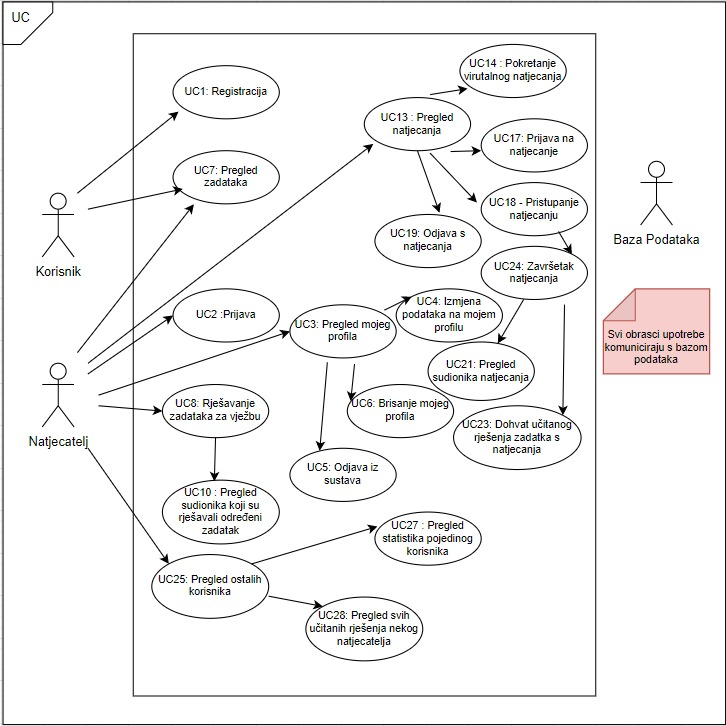
\includegraphics[width=\textwidth]{slike/DijagramObrascaUporabe1.jpeg}
					\caption{Dijagram obrasca uporabe, funkcionalnost korisnika i natjecatelja}
					\label{fig:dijaguporab1}
				\end{figure}
			\eject	

			\begin{figure}[H]
				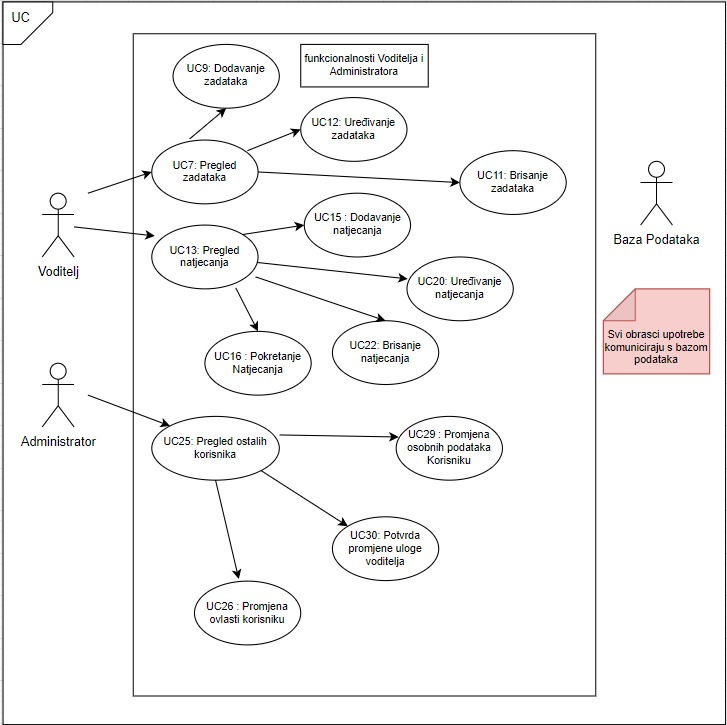
\includegraphics[width=\textwidth]{slike/DijagramObrascaUporabe2.jpeg}
				\caption{Dijagram obrasca uporabe, funkcionalnost voditelja i administratora}
				\label{fig:dijaguporab2}
			\end{figure}
		\eject	
		
				
			\subsection{Sekvencijski dijagrami}
			
				
				\subsubsection{Obrazac uporabe UC9 - Dodavanje zadataka}
				
				\noindent Voditelj šalje zahtjev za dodavanjem novog zadatka te mu se prikazuje stranica s poljima koja treba popuniti. Ta polja su naziv zadatka, broj bodova (tj. težina 1-5), vremensko ograničenje izvršavanja programa, tekst zadatka, primjeri za evaluaciju (ulaz i očekivani izlaz programa) i privatnost zadatka. Voditelj upisuje tražene podatke i sprema promjene. Ukoliko su svi upisani podaci ispravno napisani, voditelj dobiva potvrdu u obliku poruke da je uspješno stvorio zadatak, a ako su upisani podaci na neki način neispravni, voditelju se dojavljuje greška i nudi da ispravi podatke. 
				
				\begin{figure}[H]
					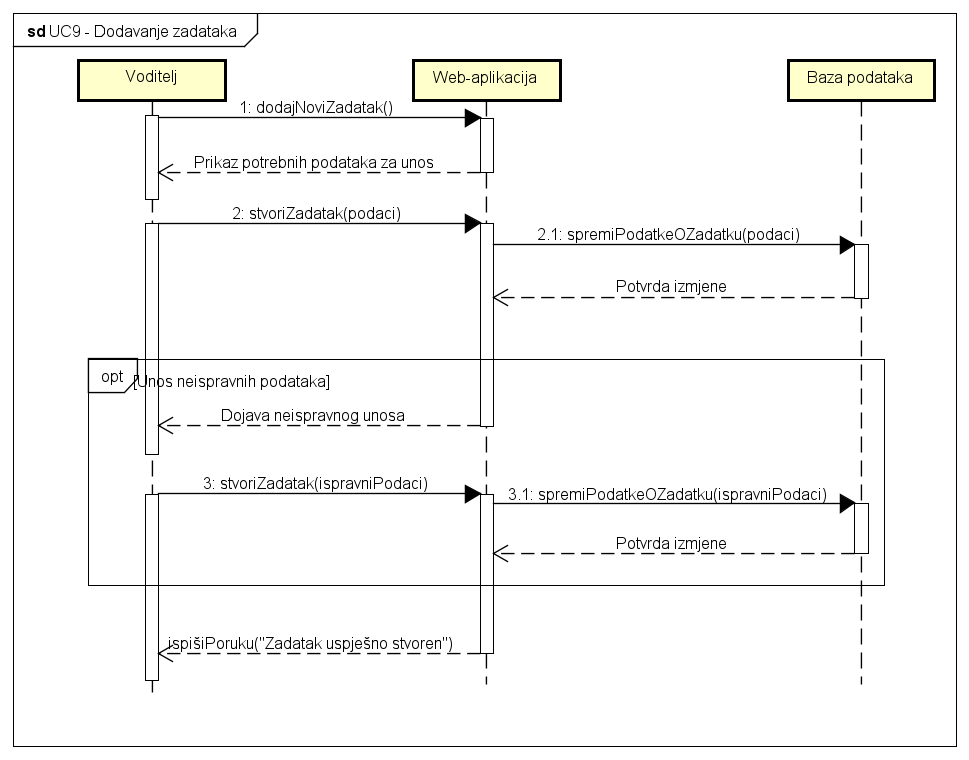
\includegraphics[width=\textwidth]{slike/SEQ_UC9.PNG}
					\caption{Sekvencijski dijagram za UC9}
					\label{fig:seq_uc9}
				\end{figure}
			\eject
				
				\subsubsection{Obrazac uporabe UC12 - Uređivanje zadataka za vježbu}
				
				\noindent Voditelj najprije odabire karticu sa zadacima te mu se prikazuje popis zadataka. Zatim odabire određeni zadatak s popisa i dobiva sve informacije o njemu. Zatim odabire opciju za uređivanje zadataka i, slično kao i u prethodnom dijagramu, prikazuje mu se stranica s istim poljima koja treba popuniti. Voditelj uređuje željene podatke, sprema promjene i, ako su uređeni podaci ispravni, dobiva potvrdu o uspješnom uređivanju zadatka, inače dobiva poruku greške i nudi mu se da ispravi podatke.
				
				\begin{figure}[H]
					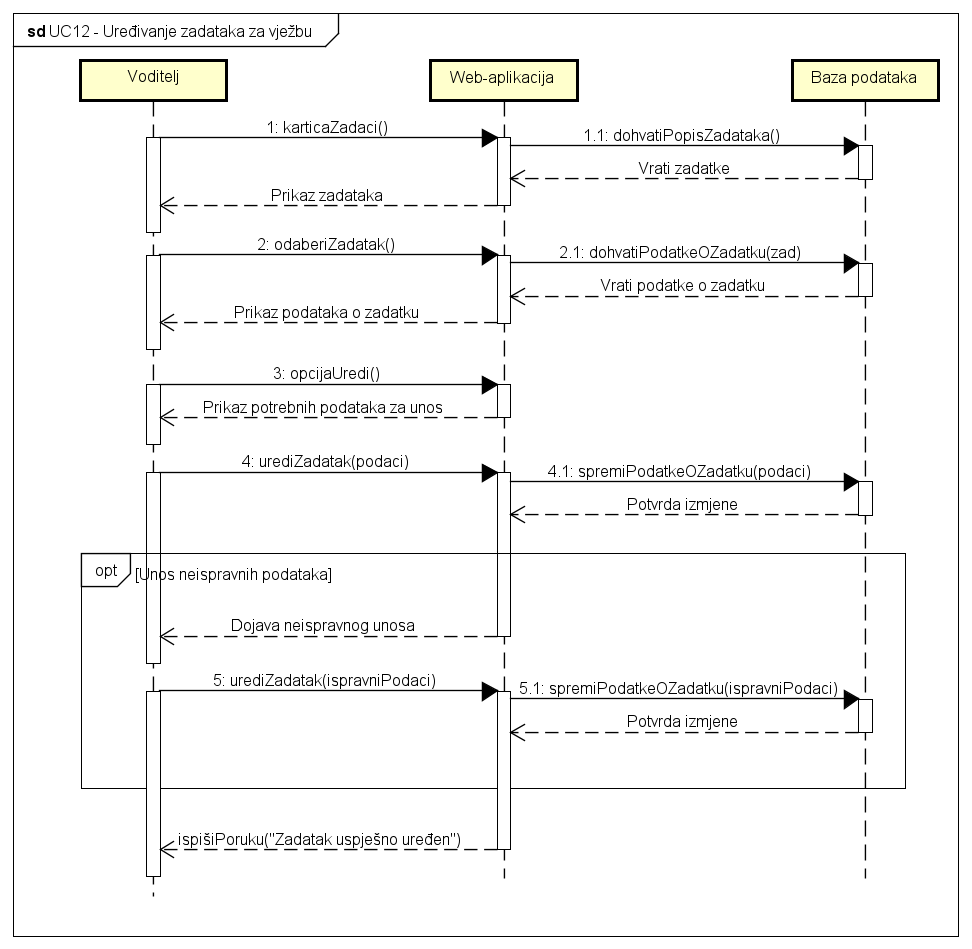
\includegraphics[width=\textwidth]{slike/SEQ_UC12.PNG}
					\caption{Sekvencijski dijagram za UC12}
					\label{fig:seq_uc12}
				\end{figure}
				\eject
				
				\subsubsection{Obrazac uporabe UC23 - Dohvat učitanog rješenja zadatka s natjecanja}
				
				\noindent Natjecatelj najprije odabire karticu s natjecanjima i dobiva popis natjecanja. Nakon toga bira željeno natjecanje i dobiva sve informacije o njemu. Zatim odabire zadatak čije rješenje želi dohvatiti i prikazuju mu se podaci o zadatku. Na ovoj stranici odabire opciju za dohvat rješenja i prima potvrdu o njegovom uspješnom preuzimanju samo ako je natjecatelj već riješio taj zadatak, i to potpuno točno, a inače dobiva poruku da ne može preuzeti rješenje tog zadatka. 
				
				\begin{figure}[H]
					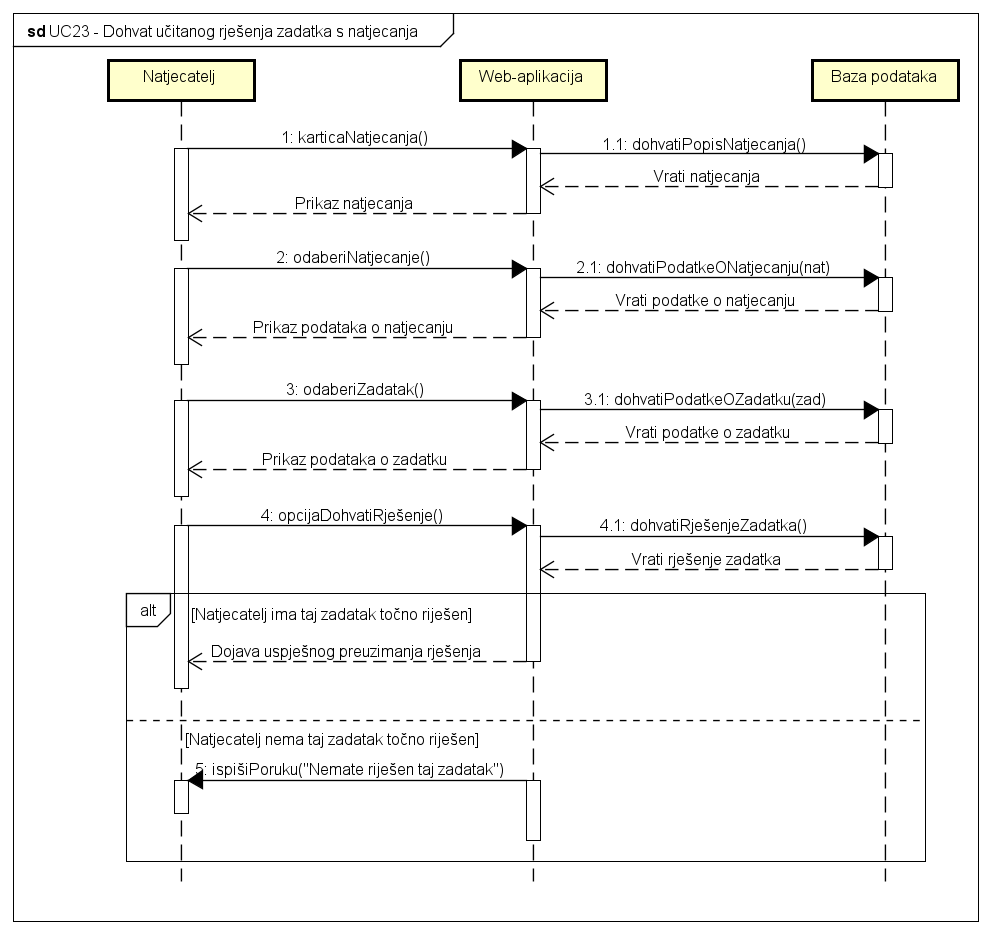
\includegraphics[width=\textwidth]{slike/SEQ_UC23.PNG}
					\caption{Sekvencijski dijagram za UC23}
					\label{fig:seq_uc23}
				\end{figure}
		\eject
	
		\section{Ostali zahtjevi}
		
		\begin{packed_item}
			\item Sustav treba omogućiti rad više korisnika u stvarnom vremenu
			 \item Korisničko sučelje i sustav moraju podržavati hrvatsku abecedu (dijakritičke znakove) pri unosu i prikazu tekstualnog sadržaja
			\item Izvršavanje dijela programa u kojem se pristupa bazi podataka ne smije trajati duže od nekoliko sekundi
			\item Sustav treba biti implementiran kao web aplikacija koristeći objektno-orijentirane jezike
			\item Neispravno korištenje korisničkog sučelja ne smije narušiti funkcionalnost i rad sustava
			\item Sustav treba biti jednostavan za korištenje, korisnici se moraju znati koristiti sučeljem bez opširnih uputa
			\item Sustav mora validirati podatke na klijentskoj i poslužiteljskoj strani
			\item Veza s bazom podataka mora biti kvalitetno zaštićena, brza i otporna na vanjske greške
			\item Pristup sustavu mora biti omogućen iz javne mreže pomoću HTTPS.
			\item Sustav je responzivan na mobilnim uređajima 
		\end{packed_item}	
			 
			 
			 
	